\documentclass[14pt]{extbook}
\usepackage{multicol, enumerate, enumitem, hyperref, color, soul, setspace, parskip, fancyhdr} %General Packages
\usepackage{amssymb, amsthm, amsmath, latexsym, units, mathtools} %Math Packages
\everymath{\displaystyle} %All math in Display Style
% Packages with additional options
\usepackage[headsep=0.5cm,headheight=12pt, left=1 in,right= 1 in,top= 1 in,bottom= 1 in]{geometry}
\usepackage[usenames,dvipsnames]{xcolor}
\usepackage{dashrule}  % Package to use the command below to create lines between items
\newcommand{\litem}[1]{\item#1\hspace*{-1cm}\rule{\textwidth}{0.4pt}}
\pagestyle{fancy}
\lhead{Progress Quiz 3}
\chead{}
\rhead{Version B}
\lfoot{3012-8528}
\cfoot{}
\rfoot{Summer C 2021}
\begin{document}

\begin{enumerate}
\litem{
Describe the end behavior of the polynomial below.\[ f(x) = 4(x + 3)^{4}(x - 3)^{9}(x + 2)^{4}(x - 2)^{6} \]\begin{enumerate}[label=\Alph*.]
\begin{multicols}{2}\item 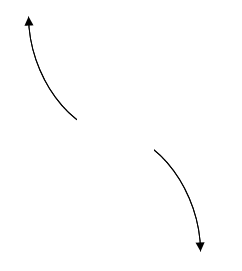
\includegraphics[width = 0.3\textwidth]{../Figures/polyEndBehaviorCopyAB.png}\item 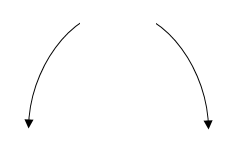
\includegraphics[width = 0.3\textwidth]{../Figures/polyEndBehaviorCopyBB.png}\item 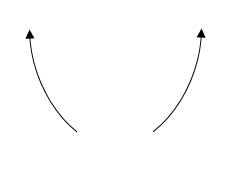
\includegraphics[width = 0.3\textwidth]{../Figures/polyEndBehaviorCopyCB.png}\item 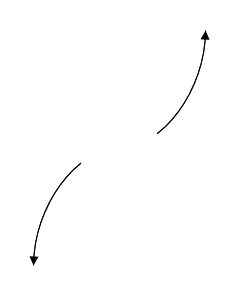
\includegraphics[width = 0.3\textwidth]{../Figures/polyEndBehaviorCopyDB.png}\end{multicols}\item None of the above.
\end{enumerate} }
\litem{
Describe the zero behavior of the zero $x = -8$ of the polynomial below.\[ f(x) = -3(x + 9)^{6}(x - 9)^{5}(x + 8)^{14}(x - 8)^{9} \]\begin{enumerate}[label=\Alph*.]
\begin{multicols}{2}\item 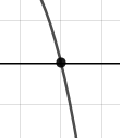
\includegraphics[width = 0.3\textwidth]{../Figures/polyZeroBehaviorAB.png}\item 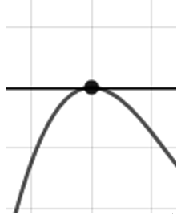
\includegraphics[width = 0.3\textwidth]{../Figures/polyZeroBehaviorBB.png}\item 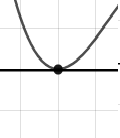
\includegraphics[width = 0.3\textwidth]{../Figures/polyZeroBehaviorCB.png}\item 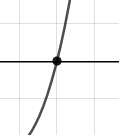
\includegraphics[width = 0.3\textwidth]{../Figures/polyZeroBehaviorDB.png}\end{multicols}\item None of the above.
\end{enumerate} }
\litem{
Which of the following equations \textit{could} be of the graph presented below?
\begin{center}
    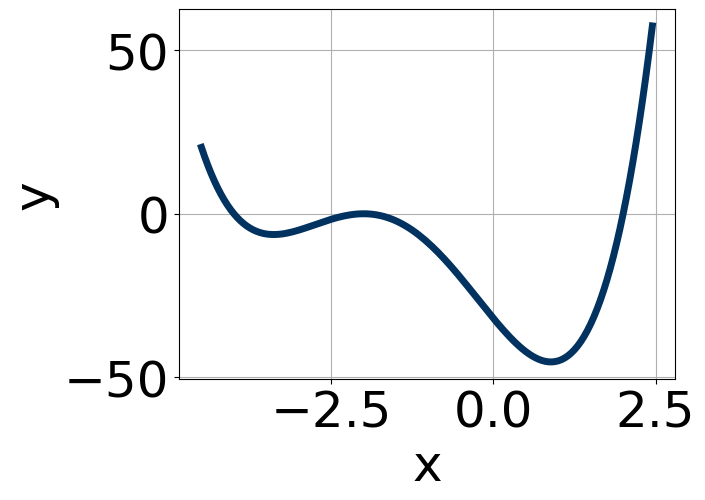
\includegraphics[width=0.5\textwidth]{../Figures/polyGraphToFunctionB.png}
\end{center}
\begin{enumerate}[label=\Alph*.]
\item \( 17(x + 2)^{10} (x - 2)^{7} (x + 4)^{5} \)
\item \( -9(x + 2)^{10} (x - 2)^{9} (x + 4)^{11} \)
\item \( -18(x + 2)^{10} (x - 2)^{11} (x + 4)^{10} \)
\item \( 8(x + 2)^{7} (x - 2)^{4} (x + 4)^{5} \)
\item \( 20(x + 2)^{4} (x - 2)^{4} (x + 4)^{9} \)

\end{enumerate} }
\litem{
Construct the lowest-degree polynomial given the zeros below. Then, choose the intervals that contain the coefficients of the polynomial in the form $x^3+bx^2+cx+d$.\[ 3 + 2 i \text{ and } 4 \]\begin{enumerate}[label=\Alph*.]
\item \( b \in [1, 8], c \in [-7.52, -6.31], \text{ and } d \in [11, 13] \)
\item \( b \in [5, 14], c \in [36.76, 37.91], \text{ and } d \in [49, 57] \)
\item \( b \in [-15, -7], c \in [36.76, 37.91], \text{ and } d \in [-52, -48] \)
\item \( b \in [1, 8], c \in [-6.57, -5.83], \text{ and } d \in [6, 9] \)
\item \( \text{None of the above.} \)

\end{enumerate} }
\litem{
Which of the following equations \textit{could} be of the graph presented below?
\begin{center}
    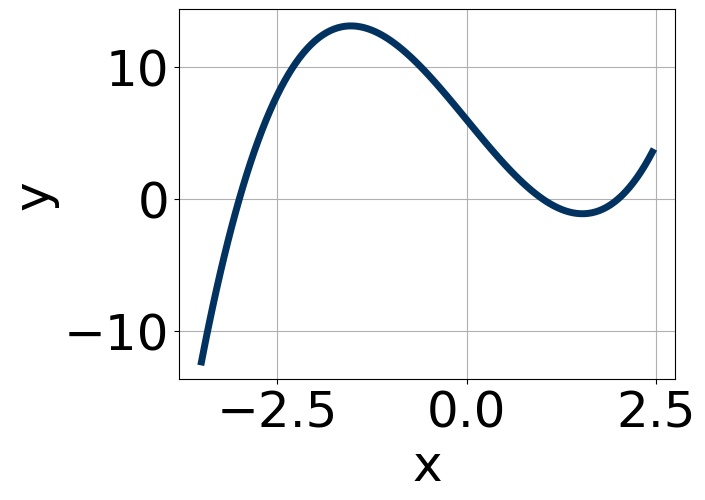
\includegraphics[width=0.5\textwidth]{../Figures/polyGraphToFunctionCopyB.png}
\end{center}
\begin{enumerate}[label=\Alph*.]
\item \( 4(x - 2)^{4} (x + 3)^{6} (x - 1)^{5} \)
\item \( 16(x - 2)^{5} (x + 3)^{5} (x - 1)^{5} \)
\item \( -9(x - 2)^{10} (x + 3)^{9} (x - 1)^{7} \)
\item \( 4(x - 2)^{6} (x + 3)^{7} (x - 1)^{11} \)
\item \( -10(x - 2)^{11} (x + 3)^{5} (x - 1)^{7} \)

\end{enumerate} }
\litem{
Describe the end behavior of the polynomial below.\[ f(x) = -9(x + 8)^{4}(x - 8)^{5}(x - 6)^{4}(x + 6)^{5} \]\begin{enumerate}[label=\Alph*.]
\begin{multicols}{2}\item 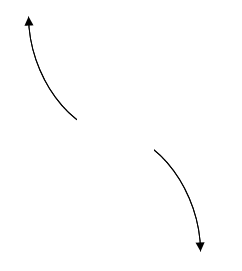
\includegraphics[width = 0.3\textwidth]{../Figures/polyEndBehaviorAB.png}\item 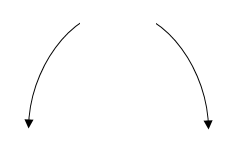
\includegraphics[width = 0.3\textwidth]{../Figures/polyEndBehaviorBB.png}\item 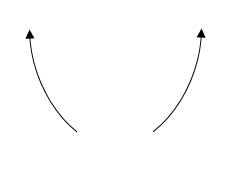
\includegraphics[width = 0.3\textwidth]{../Figures/polyEndBehaviorCB.png}\item 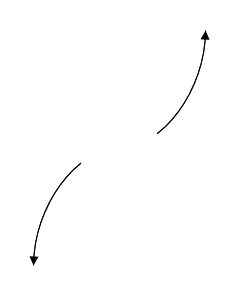
\includegraphics[width = 0.3\textwidth]{../Figures/polyEndBehaviorDB.png}\end{multicols}\item None of the above.
\end{enumerate} }
\litem{
Describe the zero behavior of the zero $x = -5$ of the polynomial below.\[ f(x) = -9(x - 5)^{4}(x + 5)^{7}(x - 9)^{4}(x + 9)^{8} \]\begin{enumerate}[label=\Alph*.]
\begin{multicols}{2}\item 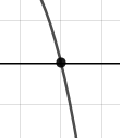
\includegraphics[width = 0.3\textwidth]{../Figures/polyZeroBehaviorCopyAB.png}\item 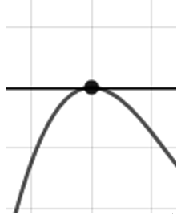
\includegraphics[width = 0.3\textwidth]{../Figures/polyZeroBehaviorCopyBB.png}\item 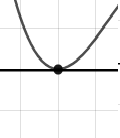
\includegraphics[width = 0.3\textwidth]{../Figures/polyZeroBehaviorCopyCB.png}\item 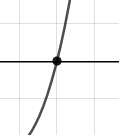
\includegraphics[width = 0.3\textwidth]{../Figures/polyZeroBehaviorCopyDB.png}\end{multicols}\item None of the above.
\end{enumerate} }
\litem{
Construct the lowest-degree polynomial given the zeros below. Then, choose the intervals that contain the coefficients of the polynomial in the form $ax^3+bx^2+cx+d$.\[ 1, \frac{-3}{4}, \text{ and } \frac{6}{5} \]\begin{enumerate}[label=\Alph*.]
\item \( a \in [20, 21], b \in [-35, -25], c \in [-9, 1], \text{ and } d \in [15, 24] \)
\item \( a \in [20, 21], b \in [-22, -14], c \in [-21, -16], \text{ and } d \in [15, 24] \)
\item \( a \in [20, 21], b \in [27, 36], c \in [-9, 1], \text{ and } d \in [-26, -17] \)
\item \( a \in [20, 21], b \in [-35, -25], c \in [-9, 1], \text{ and } d \in [-26, -17] \)
\item \( a \in [20, 21], b \in [10, 12], c \in [-33, -25], \text{ and } d \in [-26, -17] \)

\end{enumerate} }
\litem{
Construct the lowest-degree polynomial given the zeros below. Then, choose the intervals that contain the coefficients of the polynomial in the form $x^3+bx^2+cx+d$.\[ 3 + 4 i \text{ and } 4 \]\begin{enumerate}[label=\Alph*.]
\item \( b \in [-5, 7], c \in [-7.9, -4.2], \text{ and } d \in [11, 13] \)
\item \( b \in [-5, 7], c \in [-8.4, -7.9], \text{ and } d \in [13, 18] \)
\item \( b \in [7, 19], c \in [48.6, 51.5], \text{ and } d \in [98, 101] \)
\item \( b \in [-10, -4], c \in [48.6, 51.5], \text{ and } d \in [-102, -94] \)
\item \( \text{None of the above.} \)

\end{enumerate} }
\litem{
Construct the lowest-degree polynomial given the zeros below. Then, choose the intervals that contain the coefficients of the polynomial in the form $ax^3+bx^2+cx+d$.\[ \frac{3}{4}, \frac{5}{2}, \text{ and } -4 \]\begin{enumerate}[label=\Alph*.]
\item \( a \in [5, 9], b \in [16, 29], c \in [-71, -68], \text{ and } d \in [-63, -58] \)
\item \( a \in [5, 9], b \in [-13, -5], c \in [-95, -76], \text{ and } d \in [-63, -58] \)
\item \( a \in [5, 9], b \in [2, 9], c \in [-95, -76], \text{ and } d \in [55, 66] \)
\item \( a \in [5, 9], b \in [2, 9], c \in [-95, -76], \text{ and } d \in [-63, -58] \)
\item \( a \in [5, 9], b \in [57, 64], c \in [115, 125], \text{ and } d \in [55, 66] \)

\end{enumerate} }
\end{enumerate}

\end{document}